
People discovered what was wrong with classical mechanics bit by bit and, consequently, the historical development of quantum mechanics was highly ``non-linear''. Rather than following this development, we will afford the luxury of having a well-working theory of quantum mechanics, and we will present it from the foundations up. We begin by writing down a list things we would like to have. 
\subsection[Desiderata]{Desiderata\protect\footnote{Educated term for ``wishlist''.}}

A working theory of quantum mechanics would need to account for the following.

\ben[label=(\alph*)]
\item \textit{Measurements of observables, unlike in classical mechanics, don't just range over an interval $I\subseteq \R$.}

Recall that in classical mechanics an observable is a map $F\cl\Gamma\to\R$, where $\Gamma$ is the phase space of the system, typically given by the cotangent space $T^*Q$ of some configuration manifold $Q$. The map is taken to be at least continuous with respect to the standard topology on $\R$ and an appropriate topology on $\Gamma$, and hence if $\Gamma$ is connected, we have $F(\Gamma)=I\subseteq\R$.

Consider, for instance, the two-body problem. We have a potential $V(r)=-\tfrac{1}{r}$ and, assuming that the angular momentum $L$ is non-zero, the energy observable (or Hamiltonian) $H$ satisfies $H(\Gamma)=[E_{\mathrm{min}},\infty)\subset \R$.

However, measurements of the spectrum of the hydrogen atom give the following values for the energies (in electronvolts) assumed by the electron
\bse
\{-13.6\times \tfrac{1}{n^2}\mid n\in \N^+\} \cup (0,\infty).
\ese
Hence, we need to turn to new mathematics in which we can define a notion of observable that allows for a spectrum of measurement results for a quantum observable $A$ of the form 
\bse
\sigma(A)=\text{discrete part } \cup \text{ continuous part}.
\ese
An example would be the energies of the hydrogen atom
\bi{rCl}
\sigma(H) & =\ & 
\begin{tikzpicture}[baseline={($ (current bounding box.center)- (0,-6pt) $)}]
\foreach \i in {1,2,...,9,10}{
\draw[gray] (3-2/\i,0.1) -- (3-2/\i,-0.1);
}
\fill[lightgray]  (2.79,0.1) rectangle (5.5,-0.1);
\draw[->] (0,0)--(6,0);
\draw (1,-0.1) node[below=2pt]{$-13.6$ eV};
\draw (2.8,-0.1) node[below=2pt]{$0$ eV};
\end{tikzpicture}
\ei
Note that one of the parts may actually be empty. For instance, as we will later show, the simple quantum harmonic oscillator has the following energy spectrum 
\bi{rCl}
\sigma(H) & =\ & \begin{tikzpicture}[baseline={($ (current bounding box.center)- (0,-7.5pt) $)}]
\foreach \i in {2,...,9}{
\draw[gray] (0.6*\i,0.1) -- (0.6*\i,-0.1);
}
\draw (1.2,-0.1) node[below]{$\tfrac{1}{2}\hbar \omega$};
\draw (4,-0.1) node[below]{$(\tfrac{1}{2}+n)\hbar \omega$};
\draw[->] (0,0)--(6,0);
\end{tikzpicture}
\ei
while the spectrum of the position operator $Q$ is $\sigma(Q) =  \R$.

Also, the continuous part need not be connected, as is the case with spectrum of the Hamiltonian an electron in a periodic potential
\bi{rCl}
\sigma(H) & =\ & 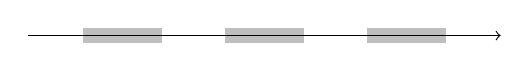
\begin{tikzpicture}
\foreach \i in {0,1,2}{
\fill[lightgray]  (1.8*\i,0.1) rectangle (1+1.8*\i,-0.1);
}
\draw[->] (-0.7,0)--(5.3,0);
\end{tikzpicture}
\ei
It turns out that self-adjoint linear maps on a complex Hilbert space provide a suitable formalism to describe the observables of quantum mechanics. 
\item \textit{An irreducible impact that each measurement has on the state of a quantum system.}

The crucial example demonstrating this is the Stern-Gerlach experiment\index{Stern-Gerlach experiment}, which consists in the following. Silver atoms are heated up in an oven and sent against a screen with a hole. The atoms passing through the hole are then subjected to an inhomogeneous magnetic field, which deflects them according to the component of their angular momentum in the direction of the field. Finally, a screen detects the various deflections.

\begin{center}
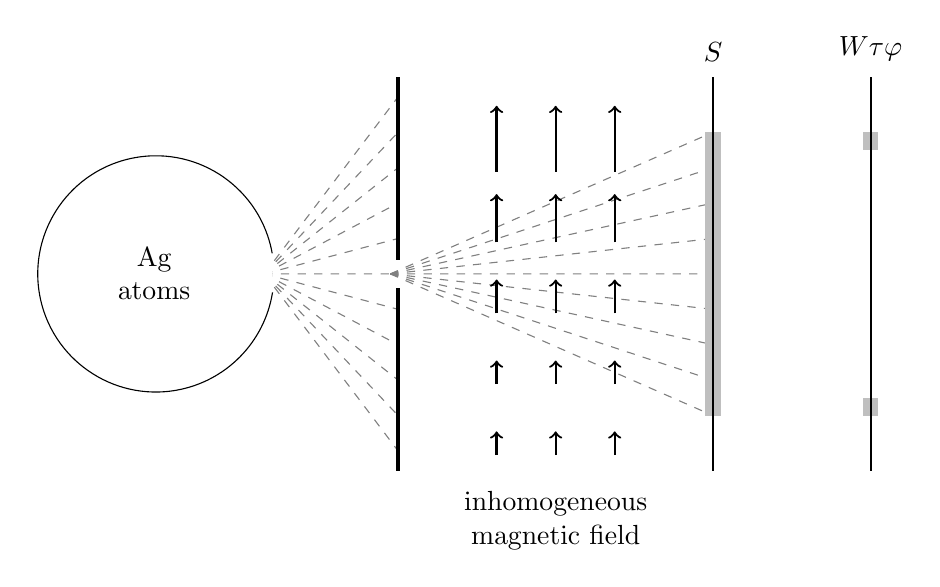
\begin{tikzpicture}[every text node part/.style={align=center}]
\foreach \i in {0,1,...,10} {
\draw[dashed,gray] (0.8,0) -- (2.5,2.25-0.45*\i);
};
\draw[fill=white] (0.9,1.5*sin 10) arc (10:351:1.5);

\draw[ultra thick] (2.5,2.5)--(2.5,0.18);
\draw[ultra thick] (2.5,-0.18)--(2.5,-2.5);
\draw (-0.6,0)  node {Ag\\ atoms};

\foreach \i in {1,...,9} {
\draw[dashed,gray] (2.4,0) -- (6.5,2.25-0.45*\i);
};

\foreach \i in {0,1,...,4} {
  \foreach \j in {1,2,3} {
\draw[thick,->] (3+0.75*\j,-2.3+0.9*\i) -- (3+0.75*\j,-2+0.9*\i^1.1);
};};

\fill[lightgray] (6.5-0.1,2.25-0.45*9) rectangle (6.5+0.1,2.25-0.45);
\draw[thick] (6.5,-2.5)--(6.5,2.5) node[above=2pt] {$S$};

\fill[lightgray] (8.5-0.1,2.25-0.45*9) rectangle (8.5+0.1,2.25-8.5*0.45);
\fill[lightgray] (8.5-0.1,2.25-0.45*1.5) rectangle (8.5+0.1,2.25-0.45);
\draw[thick] (8.5,-2.5)--(8.5,2.5) node[above=2pt] {$W\tau\varphi$};
\draw (4.5,-2.5) node[below=4pt] {inhomogeneous \\ magnetic field};
\end{tikzpicture}
\end{center}

Since the angular momentum distribution of the silver atoms coming from the oven is random, we would expect an even distribution of values of the component along the direction of the magnetic field to be recorded on the final screen, as in $S$. However, the impact pattern actually detected is that on the $W\tau\varphi$ screen. In fact, 50\% of the incoming atoms impact at the top and we say that their angular momentum component is $\uparrow$, and the other 50\% hit the bottom region, and we say that their angular momentum component is $\downarrow$.  This is another instance of our earlier point: there seem to be only two possible values for the component of angular momentum along the direction of the magnetic field, i.e.\ the spectrum is discrete. Hence, this is not particularly surprising at this point.

Let us now consider successive iterations of this experiment. Introduce some system of cartesian coordinates $(x,y,z)$ and let $\mathrm{SG}(x)$ and $\mathrm{SG}(z)$ denotes a Stern-Gerlach apparatus whose magnetic field points in the $x$ and $z$-direction, respectively.

Suppose that we sent the atoms through a first $\mathrm{SG}(z)$ apparatus, and then we use the $z^\uparrow$-output as the input of a second $\mathrm{SG}(z)$ apparatus.
\begin{center}
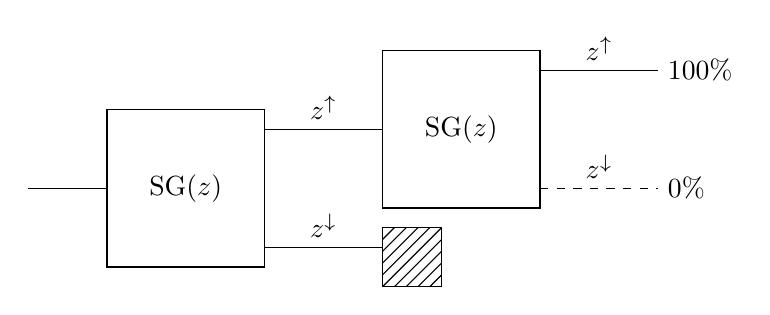
\begin{tikzpicture}[scale=0.5]
\draw (-2,2) -- (0,2);
\draw (2,2) node {$\mathrm{SG}(z)$};
\draw  (0,0) rectangle (4,4);
\draw (4,3.5) -- (7,3.5) node[above,midway] {$z^\uparrow$};
\draw (4,0.5) -- (7,0.5) node[above,midway] {$z^\downarrow$};
\draw  (7,1.5) rectangle (11,5.5);
\draw  (7,1) rectangle (8.5,-0.5);
\draw  (11,5) -- (14,5)  node[above,midway] {$z^\uparrow$} node[right] {100\%};
\draw[dashed]  (11,2) -- (14,2) node[above,midway] {$z^\downarrow$} node[right] {0\%};
\node at (9,3.5) {$\mathrm{SG}(z)$};
\foreach \i in {1,...,5} {
\draw (7+0.3*\i,1)--(7,1-0.3*\i);
\draw (7+0.3*\i,-0.5)--(8.5,1-0.3*\i);
};
\end{tikzpicture}
\end{center}
The second $\mathrm{SG}(z)$ apparatus finds no $z^\downarrow$-atoms. This is not surprising since, intuitively, we ``filtered out'' all the $z^\downarrow$-atoms with the first apparatus. Suppose now that we feed the $z^\uparrow$ output of a $\mathrm{SG}(z)$ apparatus into a $\mathrm{SG}(x)$ apparatus.

\begin{center}
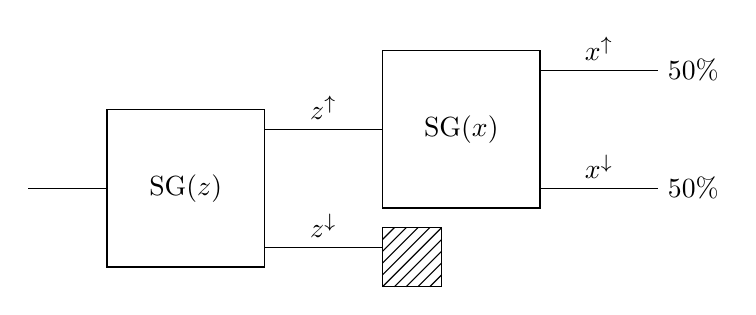
\begin{tikzpicture}[scale=0.5]
\draw (-2,2) -- (0,2);
\draw (2,2) node {$\mathrm{SG}(z)$};
\draw  (0,0) rectangle (4,4);
\draw (4,3.5) -- (7,3.5) node[above,midway] {$z^\uparrow$};
\draw (4,0.5) -- (7,0.5) node[above,midway] {$z^\downarrow$};
\draw  (7,1.5) rectangle (11,5.5);
\draw  (7,1) rectangle (8.5,-0.5);
\draw  (11,5) -- (14,5)  node[above,midway] {$x^\uparrow$} node[right] {50\%};
\draw  (11,2) -- (14,2) node[above,midway] {$x^\downarrow$} node[right] {50\%};
\node at (9,3.5) {$\mathrm{SG}(x)$};
\foreach \i in {1,...,5} {
\draw (7+0.3*\i,1)--(7,1-0.3*\i);
\draw (7+0.3*\i,-0.5)--(8.5,1-0.3*\i);
};
\end{tikzpicture}
\end{center}
Experimentally, we find that about half of the atoms are detected in the state $x^\uparrow$ and half in the state $x^\downarrow$. This is, again, not surprising since we only filtered out the $z^\uparrow$ atoms, and hence we can interpret this result as saying that the $x^\uparrow$, $x^\downarrow$ states are independent from the $z^\uparrow$, $z^\downarrow$.

If our ideas of ``filtering states out'' is correct, then feeding the $x^\uparrow$-output of the previous set-up to another $\mathrm{SG}(z)$ apparatus should clearly produce a $100\%$ $z^\uparrow$-output, since we already filtered out all the $z^\downarrow$ ones in the previous step.

\begin{center}
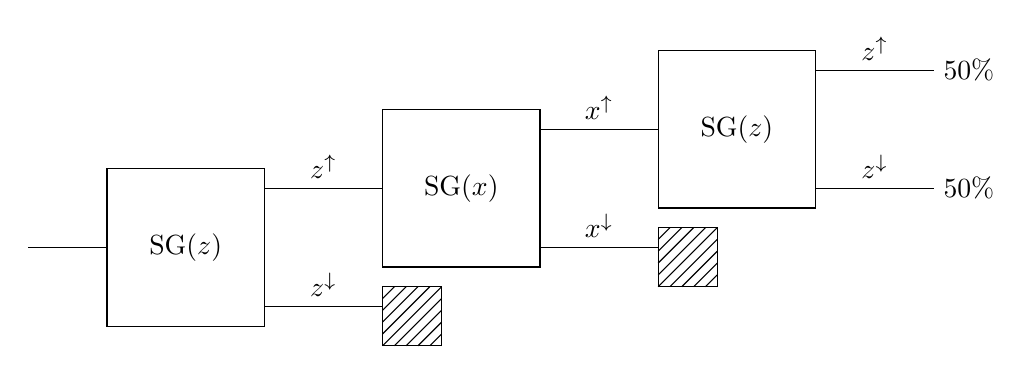
\begin{tikzpicture}[scale=0.5]
\draw (-2,2) -- (0,2);
\draw (2,2) node {$\mathrm{SG}(z)$};
\draw  (0,0) rectangle (4,4);
\draw (4,3.5) -- (7,3.5) node[above,midway] {$z^\uparrow$};
\draw (4,0.5) -- (7,0.5) node[above,midway] {$z^\downarrow$};
\draw  (7,1.5) rectangle (11,5.5);
\draw  (11,5) -- (14,5)  node[above,midway] {$x^\uparrow$} ;
\draw  (11,2) -- (14,2) node[above,midway] {$x^\downarrow$};
\node at (9,3.5) {$\mathrm{SG}(x)$};
\draw  (7,1) rectangle (8.5,-0.5);
\foreach \i in {1,...,5} {
\draw (7+0.3*\i,1)--(7,1-0.3*\i);
\draw (7+0.3*\i,-0.5)--(8.5,1-0.3*\i);
};

\draw  (14,2.5) rectangle (15.5,1);
\foreach \i in {1,...,5} {
\draw (14+0.3*\i,2.5)--(14,2.5-0.3*\i);
\draw (14+0.3*\i,2-1)--(15.5,2.5-0.3*\i);
};
\draw  (14,3) rectangle (18,7);
\draw (16,5) node {$\mathrm{SG}(z)$};
\draw (18,6.5) -- (21,6.5) node[above,midway] {$z^\uparrow$} node[right] {50\%};
\draw (18,3.5) -- (21,3.5) node[above,midway] {$z^\downarrow$} node[right] {50\%};
\end{tikzpicture}
\end{center}
Surprisingly, the output is again $50$-$50$. The idea behind this result is the following. The $\mathrm{SG}(z)$ apparatus left the atoms in a state such that a repeated measurement with the $\mathrm{SG}(z)$ apparatus would give the same result, and similarly for the $\mathrm{SG}(x)$ apparatus. However, the measurement of the $\mathrm{SG}(x)$ apparatus somehow altered the state of the atoms in such a way as to ``reset'' them with respect to a measurement by the $\mathrm{SG}(z)$ apparatus. For more details on the Stern-Gerlach experiment and  further conclusions one can draw from its results, you should consult the book \textit{Modern Quantum Mechanics} by J. J. Sakurai. The conclusion that we are interested in here is that measurements can alter the state of a system.

\item \textit{Even if the state $\rho$ of a quantum system is completely known, the only prediction one can make for the measurement of some observable $A$ is the probability that the measured valued, which is an element of the spectrum $\sigma(A)$, lies within a Borel-measurable subset $E\subseteq \R$, denoted by
$\mu^A_{\rho}(E)$}.

In particular, one cannot predict which concrete outcome an isolated measurement will produce. This is even more annoying given that the precise impact that a measurement has on the state of the system (see previous point) depends on the observed outcome of the measurement.
\een

A suitable theory that accommodates all known experimental facts has been developed between 1900 and 1927 on the physics side by, among others, Schr\"odinger, Heisenberg and Dirac, and on the mathematical side almost single-handedly by von Neumann who invented a massive proportion of a field known today as functional analysis.

\subsection{The axioms of quantum mechanics}

We will now present the axioms of quantum mechanics by using notions and terminology that will be defined later in the course. In this sense, this section constitutes a preview of the next few lectures. 

\begin{tcolorbox}[colframe=blue!10!black,before skip=10pt,after skip=10pt]
\begin{axiom}[Quantum systems and states]
To every quantum system there is associated a separable complex Hilbert space $(\mathcal{H},+,\cdot,\langle \cdot | \cdot \rangle)$. The states of the system are all positive, trace-class linear maps $\rho\cl \mathcal{H}\to \mathcal{H}$ for which $\Tr\rho=1$.
\end{axiom}
\end{tcolorbox}

\br
Throughout the quantum mechanics literature, it is stated that the unit, or normalised, elements $\psi\in\mathcal{H}$ (that is, $\langle\psi|\psi\rangle=1$) are the states of the quantum system. This is not correct. 

States can be pure or mixed. A state $\rho\cl \mathcal{H}\to \mathcal{H}$ is called \emph{pure} if
\bse
\exists \, \psi\in \mathcal{H} : \forall \, \alpha\in \mathcal{H} : \ \rho(\alpha) = \frac{\langle\psi|\alpha\rangle}{\langle\psi|\psi\rangle}\psi.
\ese
Thus, we can associate to each pure state $\rho$ an element $\psi\in\mathcal{H}$. However, this correspondence is not one-to-one. Even if we restrict to pure states and impose the normalisation condition, there can be many $\psi\in\mathcal{H}$ representing the same pure state $\rho$. 

Therefore, it is wrong to say that the states of the states of the quantum system are the normalised elements of the Hilbert space, since they do not represent all the states of the system, and do not even represent uniquely the states that they do represent.
\er

The terms used in Axiom 1 are defined as follows.

\bd
A \emph{complex Hilbert space}\index{Hilbert space} is a tuple $(\mathcal{H},+,\cdot,\langle \cdot | \cdot \rangle)$ where
\begin{itemize}
\item $\mathcal{H}$ is a set
\item $+$ is a map $+\cl\mathcal{H}\times \mathcal{H}\to \mathcal{H}$
\item $\cdot$ is a map $\cdot \cl \C \times \mathcal{H}\to \mathcal{H}$ (typically suppressed in the notation)
\end{itemize}
such that the triple $(\mathcal{H},+,\cdot)$ is a vector space over $\C$, and
\begin{itemize}
\item $\langle \cdot | \cdot \rangle$ is a \emph{sesqui-linear\footnote{sesqui is Latin for ``one and a half''.}inner product}, i.e.\ a map $\langle \cdot | \cdot \rangle\cl\mathcal{H}\times \mathcal{H}\to \mathcal{H}$ satisfying
\ben[label=(\roman*)]
\item $\langle \varphi|\psi\rangle=\overline{\langle \psi|\varphi\rangle}$\hfill (conjugate symmetry/Hermitian property)
\item $\langle \varphi|z\psi_1+\psi_2\rangle=z\langle \varphi|\psi_1\rangle+\langle \varphi|\psi_2\rangle$ \hfill (linearity in the second argument)
\item $\langle \psi | \psi\rangle \geq 0$ and $\langle \psi|\psi\rangle = 0 \Leftrightarrow \psi = 0$ \hfill (positive-definiteness)
\een
for all $\varphi,\psi_1,\psi_2\in\mathcal{H}$ and $z\in \C$,
\end{itemize}
and moreover
\begin{itemize}
\item $\mathcal{H}$ is a \emph{complete metric space} with respect to the metric induced by the norm induced in turn by the sesqui-linear map $\langle \cdot | \cdot \rangle$. Explicitly, for every sequence $\phi\cl \N \to \mathcal{H}$ that satisfies the \emph{Cauchy property}, namely
\bse
\forall \, \varepsilon > 0 : \exists \, N\in \N : \forall \, n,m \geq N : \ \|\phi_n-\phi_m\|< \varepsilon,
\ese
where $\phi_n:=\phi(n)$ and $\|\psi\|:=\sqrt{\langle \psi | \psi \rangle}$, then the sequence converges in $\mathcal{H}$, i.e.\
\bse
\exists \, \varphi\in\mathcal{H}:\forall \, \varepsilon > 0 : \exists \, N\in \N : \forall \, n \geq N : \ \|\varphi-\phi_n\|< \varepsilon.
\ese
\end{itemize}
\ed
Note that the $\C$-vector space $(\mathcal{H},+,\cdot)$ need not be finite-dimensional and, in fact, we will mostly work with infinite-dimensional Hilbert spaces. 

\bd
A map $A\cl\mathcal{D}_A\to \mathcal{H}$, where the subspace $\mathcal{D}_A\subseteq \mathcal{H}$ is called the \emph{domain} of $A$, is a \emph{linear map} if
\bse
\forall \, \varphi,\psi\in\mathcal{D}_A:\forall \, z \in \C : \ A(z\varphi+\psi)=zA(\varphi)+A(\psi).
\ese
\ed
From now on, if there is no risk of confusion, we will write $A\varphi:=A(\varphi)$ in order to spare some brackets. We will be particularly interested in special types of linear map.


% \bd
% A linear map $A\cl\mathcal{D}_A\to \mathcal{H}$ is said to be
% \begin{itemize}
% \item \emph{densely defined} if $\mathcal{D}_A$ is \emph{dense} in $\mathcal{H}$, i.e.\
% \bse
% \forall \, \psi\in \mathcal{H} : \exists \, \alpha \in \mathcal{D}_A : \forall \, \varepsilon >0 :\ \|\alpha-\psi\|<\varepsilon
% \ese
% \item \emph{positive} if 
% \bse
% \forall \, \psi\in\mathcal{D}_A : \ \langle\psi|A\psi\rangle\geq 0
% \ese
% \item of \emph{trace-class} if $\mathcal{D}_A=\mathcal{H}$ and, for any orthonormal basis $\{e_n\}$ of $\mathcal{H}$, the sum/series
% \bse
% \sum_n \langle e_n|Ae_n\rangle < \infty.
% \ese
% \end{itemize}
% \ed


\bd
A linear map $A\cl\mathcal{D}_A\to \mathcal{H}$ is \emph{densely defined} if $\mathcal{D}_A$ is \emph{dense} in $\mathcal{H}$, i.e.\
\bse
\forall \, \psi\in \mathcal{H} : \forall \, \varepsilon >0: \exists \, \alpha \in \mathcal{D}_A  :\ \|\alpha-\psi\|<\varepsilon.
\ese
\ed

\bd
A linear map $A\cl\mathcal{D}_A\to \mathcal{H}$ is said to be \emph{positive} if 
\bse
\forall \, \psi\in\mathcal{D}_A : \ \langle\psi|A\psi\rangle\geq 0.
\ese
\ed


\bd
A linear map $A\cl\mathcal{D}_A\to \mathcal{H}$ is said to be of \emph{trace-class} if $\mathcal{D}_A=\mathcal{H}$ and, for any orthonormal basis $\{e_n\}$ of $\mathcal{H}$, the sum/series
\bse
\sum_n \langle e_n|Ae_n\rangle < \infty.
\ese
\ed
If $A\cl\mathcal{H}\to \mathcal{H}$ is of trace-class, one can show that the value of $\sum_n \langle e_n|Ae_n\rangle$ does not depend on the choice of orthonormal basis $\{e_n\}$. 
\bd
Let $A\cl\mathcal{H}\to \mathcal{H}$ be of trace-class. Then the \emph{trace} of $A$ is
\bse
\Tr A :=\sum_n \langle e_n|Ae_n\rangle 
\ese
where $\{e_n\}$ is any orthonormal basis of $\mathcal{H}$.
\ed
\begin{tcolorbox}[colframe=blue!10!black]
\begin{axiom}[Observables]
The observables of a quantum system are the self-adjoint linear maps $A\cl\mathcal{D}_A\to \mathcal{H}$.
\end{axiom}
\end{tcolorbox}
While the notion of a self-adjoint map is easy to define in finite-dimensional spaces, it is much more subtle for infinite-dimensional spaces.

\bd
A densely defined linear map $A\cl\mathcal{D}_A\to \mathcal{H}$ is said to be of \emph{self-adjoint} if it coincides with its adjoint map $A^*\cl\mathcal{D}_{A^*}\to \mathcal{H}$, that is
\begin{itemize}
\item $\mathcal{D}_A=\mathcal{D}_{A^*}$
\item $\forall \, \varphi\in\mathcal{D}_A : \ A\varphi=A^*\varphi$.
\end{itemize}
\ed
%The subtle part is the definition of the adjoint map itself.
\bd
The \emph{adjoint map} $A^*\cl\mathcal{D}_{A^*}\to \mathcal{H}$ of a linear map $A\cl\mathcal{D}_A\to \mathcal{H}$ is defined by
\begin{itemize}
\item $\mathcal{D}_{A^*}:=\{\psi\in\mathcal{H}\mid \forall \, \alpha \in \mathcal{D}_A:\exists \, \eta \in \mathcal{H} : \langle\psi|A\alpha\rangle=\langle\eta|\alpha\rangle\}$
\item $A^*\psi:=\eta$.
\end{itemize}
\ed
We will later show that the adjoint map is well-defined, i.e.\ for each $\alpha\in\mathcal{D}_A$ and $\psi\in\mathcal{H}$ there exists at most one $\eta\in\mathcal{H}$ such that $\langle\psi|A\alpha\rangle = \langle\eta|\alpha\rangle$.

\br
If we defined $\mathcal{D}_{A^*}$ by requiring that $\eta\in \mathcal{D}_{A}$, we would obtain a notion of self-adjointness which has undesirable properties. In particular, the spectrum (to be defined later) of a self-adjoint operator would not be guaranteed to be a subset of $\R$.
\er

\begin{tcolorbox}[colframe=blue!10!black]
\begin{axiom}[Measurement]
The probability that a measurement of an observable $A$ on a system that is in the state $\rho$ yields a result in the Borel set $E\subseteq \R$ is given by
\bse
\mu^A_\rho(E):=\Tr(\mathrm{P}_{\!A}(E)\circ\rho)
\ese
where the map $\mathrm{P}_{\!A}\cl \Borel(\R)\to\mathcal{L}(\mathcal{H})$, from the Borel-measurable subsets of $\R$ to the Banach space of bounded linear maps on $\mathcal{H}$, is the unique projection-valued measure that is associated with the self-adjoint map $A$ according to the spectral theorem.\end{axiom}\end{tcolorbox}

We will later see that the composition of a bounded linear map with a trace-class map is again of trace-class, so that $\Tr(\mathrm{P}_{\!A}(E)\circ\rho)$ is well-defined. For completeness, the spectral theorem states that for any self-adjoint map $A$ there exists a projection-valued measure $\mathrm{P}_{\!A}$ such that $A$ can be represented in terms of the Lebesgue-Stieltjes integral as
\bse
A = \int_{\R}\lambda \, \d \mathrm{P}_{\!A}(\lambda).
\ese
This is the infinite-dimensional analogue of the diagonalisation theorem for symmetric or Hermitian matrices on finite-dimensional vector spaces, and it is the theorem in which the first half of the course will find its climax.


\begin{tcolorbox}[colframe=blue!10!black,before skip=10pt]
\begin{axiom}[Unitary dynamics]
In a time interval $(t_1,t_2)\subseteq \R$ in which no measurement occurs, the state $\rho$ at time $t_1$, denoted $\rho(t_1)$, is related to the state $\rho$ at time $t_2$, denoted $\rho(t_2)$, by
\bse
\rho(t_2) = \mathcal{U}(t_2-t_1)\rho(t_1)\mathcal{U}^{-1}(t_2-t_1)
\ese
with the unitary evolution operator $\mathcal{U}$ defined as
\bse
\mathcal{U}(t) := \exp(-\tfrac{\mathrm{i}}{\hbar}Ht),
\ese
where $H$ is the energy observable and, for any observable $A$ and $f\cl \R\to \C$, we define
\bse
f(A):=\int_\R f(\lambda) \, \d \mathrm{P}_{\!A}(\lambda).
\ese
\end{axiom}
\end{tcolorbox}
Note that, as was the case for the previous axiom, the spectral theorem is crucial since it is needed to define  the unitary evolution operator.

\begin{tcolorbox}[colframe=blue!10!black,before skip=10pt]
\begin{axiom}[Projective dynamics]
The state $\rho_{\mathrm{after}}$ of a quantum system immediately following the measurement of an observable $A$ is
\bse
\rho_{\mathrm{after}} := \frac{\mathrm{P}_{\!A}(E)\circ\rho_{\mathrm{before}}\circ\mathrm{P}_{\!A}(E)}{\Tr(\mathrm{P}_{\!A}(E)\circ\rho_{\mathrm{before}}\circ\mathrm{P}_{\!A}(E))}
\ese
where $\rho_{\mathrm{before}}$ is the state immediately preceding the measurement and $E\subseteq\R$ is the smallest Borel set in which the actual outcome of the measurement happened to lie.
\end{axiom}
\end{tcolorbox}























